% -*- mode: latex; mode: flyspell; ispell-local-dictionary: "en_US"; coding: utf-8; fill-column: 80 -*-

\documentclass{article}

\usepackage[utf8]{inputenc}
\usepackage[english]{babel}

\usepackage{amsmath,amsfonts,amssymb}
\usepackage{fullpage}
\usepackage{verbatim}

\usepackage{tikz,pgfplots}

\pgfplotsset{
  width=150mm,height=100mm,
  major grid style={thin,dotted,color=black!50},
  minor grid style={thin,dotted,color=black!50},
  grid,
  every axis/.append style={
    line width=0.5pt,
    tick style={
      line cap=round,
      thin,
      major tick length=4pt,
      minor tick length=2pt,
    },
  },
  legend cell align=left,
  legend pos=north west,
}

%%%%%%%%%%%%%%%%%%%%%%%%%%%%%%%%%%%%%%%%%%%%%%%%%%%%%%%%%%%%%%%%%%%%%%%%%%%%%%%%

\begin{document}

\title{Hashmap Sizes}
\author{}
\maketitle


% IMPORT-DATA mphf stats_mphf_size.txt


\begin{center}
	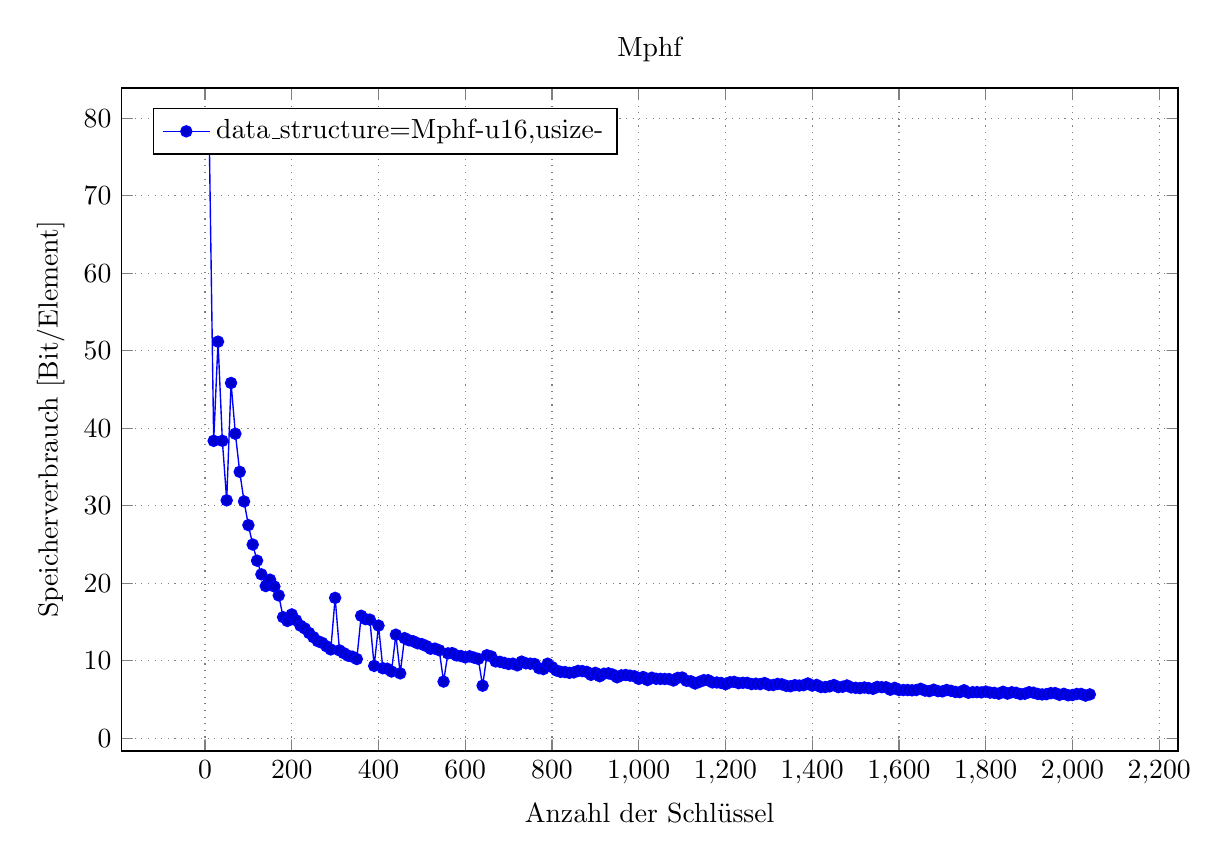
\begin{tikzpicture}
	\begin{axis}[
	title={Mphf},
	xlabel={Anzahl der Schlüssel},
	ylabel={Speicherverbrauch [Bit/Element]},
	]
	
	%% MULTIPLOT(data_structure) SELECT size AS x, size_bytes AS y, MULTIPLOT
	%% FROM mphf GROUP BY MULTIPLOT,x ORDER BY MULTIPLOT,x
 \addplot coordinates { (10,76.8) (20,38.4) (30,51.2) (40,38.4) (50,30.72) (60,45.8667) (70,39.3143) (80,34.4) (90,30.5778) (100,27.52) (110,25.0182) (120,22.9333) (130,21.1692) (140,19.6571) (150,20.48) (160,19.6) (170,18.4471) (180,15.6444) (190,15.1579) (200,16.0) (210,15.2381) (220,14.5455) (230,14.1913) (240,13.6) (250,13.056) (260,12.5538) (270,12.3259) (280,11.8857) (290,11.4759) (300,18.1333) (310,11.3548) (320,11.0) (330,10.6667) (340,10.5412) (350,10.24) (360,15.8222) (370,15.3946) (380,15.3263) (390,9.35385) (400,14.56) (410,9.05366) (420,8.99048) (430,8.63256) (440,13.3818) (450,8.39111) (460,12.9391) (470,12.6638) (480,12.5333) (490,12.2776) (500,12.16) (510,11.9216) (520,11.5692) (530,11.5925) (540,11.3778) (550,7.33091) (560,10.9714) (570,11.0035) (580,10.7034) (590,10.6305) (600,10.4533) (610,10.5967) (620,10.4258) (630,10.2603) (640,6.8) (650,10.7323) (660,10.5697) (670,9.93433) (680,9.88235) (690,9.73913) (700,9.6) (710,9.64507) (720,9.42222) (730,9.90685) (740,9.68649) (750,9.64267) (760,9.6) (770,9.05974) (780,8.94359) (790,9.64051) (800,9.2) (810,8.77037) (820,8.58537) (830,8.55904) (840,8.45714) (850,8.50824) (860,8.70698) (870,8.68046) (880,8.58182) (890,8.19775) (900,8.46222) (910,8.01758) (920,8.34783) (930,8.3957) (940,8.2383) (950,7.88211) (960,8.13333) (970,8.18144) (980,8.09796) (990,8.01616) (1000,7.68) (1010,7.92079) (1020,7.52941) (1030,7.82913) (1040,7.69231) (1050,7.68) (1060,7.66792) (1070,7.65607) (1080,7.46667) (1090,7.80917) (1100,7.85455) (1110,7.43784) (1120,7.37143) (1130,7.07965) (1140,7.29825) (1150,7.51304) (1160,7.50345) (1170,7.22051) (1180,7.21356) (1190,7.15294) (1200,6.98667) (1210,7.24628) (1220,7.2918) (1230,7.12846) (1240,7.17419) (1250,7.168) (1260,7.00952) (1270,7.05512) (1280,7.0) (1290,7.14419) (1300,6.89231) (1310,6.88855) (1320,7.0303) (1330,6.97744) (1340,6.78209) (1350,6.73185) (1360,6.87059) (1370,6.82044) (1380,6.86377) (1390,7.09065) (1400,6.81143) (1410,6.89929) (1420,6.62535) (1430,6.62378) (1440,6.71111) (1450,6.88552) (1460,6.61918) (1470,6.66122) (1480,6.83243) (1490,6.57181) (1500,6.528) (1510,6.48477) (1520,6.56842) (1530,6.48366) (1540,6.4) (1550,6.64774) (1560,6.60513) (1570,6.60382) (1580,6.27848) (1590,6.52075) (1600,6.24) (1610,6.24099) (1620,6.24198) (1630,6.20368) (1640,6.2439) (1650,6.4) (1660,6.16867) (1670,6.09341) (1680,6.28571) (1690,6.09704) (1700,6.06118) (1710,6.25029) (1720,6.13953) (1730,5.99306) (1740,5.95862) (1750,6.21714) (1760,5.89091) (1770,5.9661) (1780,5.96854) (1790,5.9352) (1800,6.04444) (1810,5.90497) (1820,5.87253) (1830,5.77049) (1840,6.01739) (1850,5.7773) (1860,5.95269) (1870,5.88663) (1880,5.71915) (1890,5.75661) (1900,5.96211) (1910,5.89738) (1920,5.73333) (1930,5.67047) (1940,5.70722) (1950,5.84205) (1960,5.8449) (1970,5.6203) (1980,5.75354) (1990,5.56382) (2000,5.6) (2010,5.73134) (2020,5.73465) (2030,5.51724) (2040,5.67843) };
 \addlegendentry{data\_structure=Mphf-u16,usize-};
 
	
	\end{axis}
	\end{tikzpicture}
\end{center}


\end{document}

%%%%%%%%%%%%%%%%%%%%%%%%%%%%%%%%%%%%%%%%%%%%%%%%%%%%%%%%%%%%%%%%%%%%%%%%%%%%%%%%
